% ------------------------------------------------------------------------------
% 7.2. DIAGRAMA DE CLASE
% ------------------------------------------------------------------------------
\subsection{7.2. Diagrama de Clase}\label{sec:cap7_diagrama_clase}

El diagrama de clases de diseño integra las clases de entidad identificadas en el análisis de los casos de uso (Capítulo 6) y las refina con sus atributos, tipos de datos, operaciones y relaciones de asociación, composición y herencia, expresadas en el Lenguaje Unificado de Modelado \parencite{booch2005uml}. Las clases representan la información persistente del dominio de la Beca Comedor y se corresponden con las tablas del diseño de datos (sección~\ref{sec:cap7_diseno_datos}); los valores admitidos para los estados y tipos se modelan como enumeraciones.

Todas las clases, excepto \textit{Postulante}, que hereda de \textit{Usuario}, heredan de la clase abstracta \textit{EntidadBase}, que aporta el identificador interno, el código público (UUID) y las fechas de creación, actualización y eliminación lógica; las líneas de esa herencia se omiten en el diagrama para no saturarlo. La Figura~\ref{fig:diagrama_clases} presenta el diagrama de clases del sistema.

\begin{landscape}
\begin{figure}[p]
\caption{Diagrama de clases del sistema}
\label{fig:diagrama_clases}
\centering
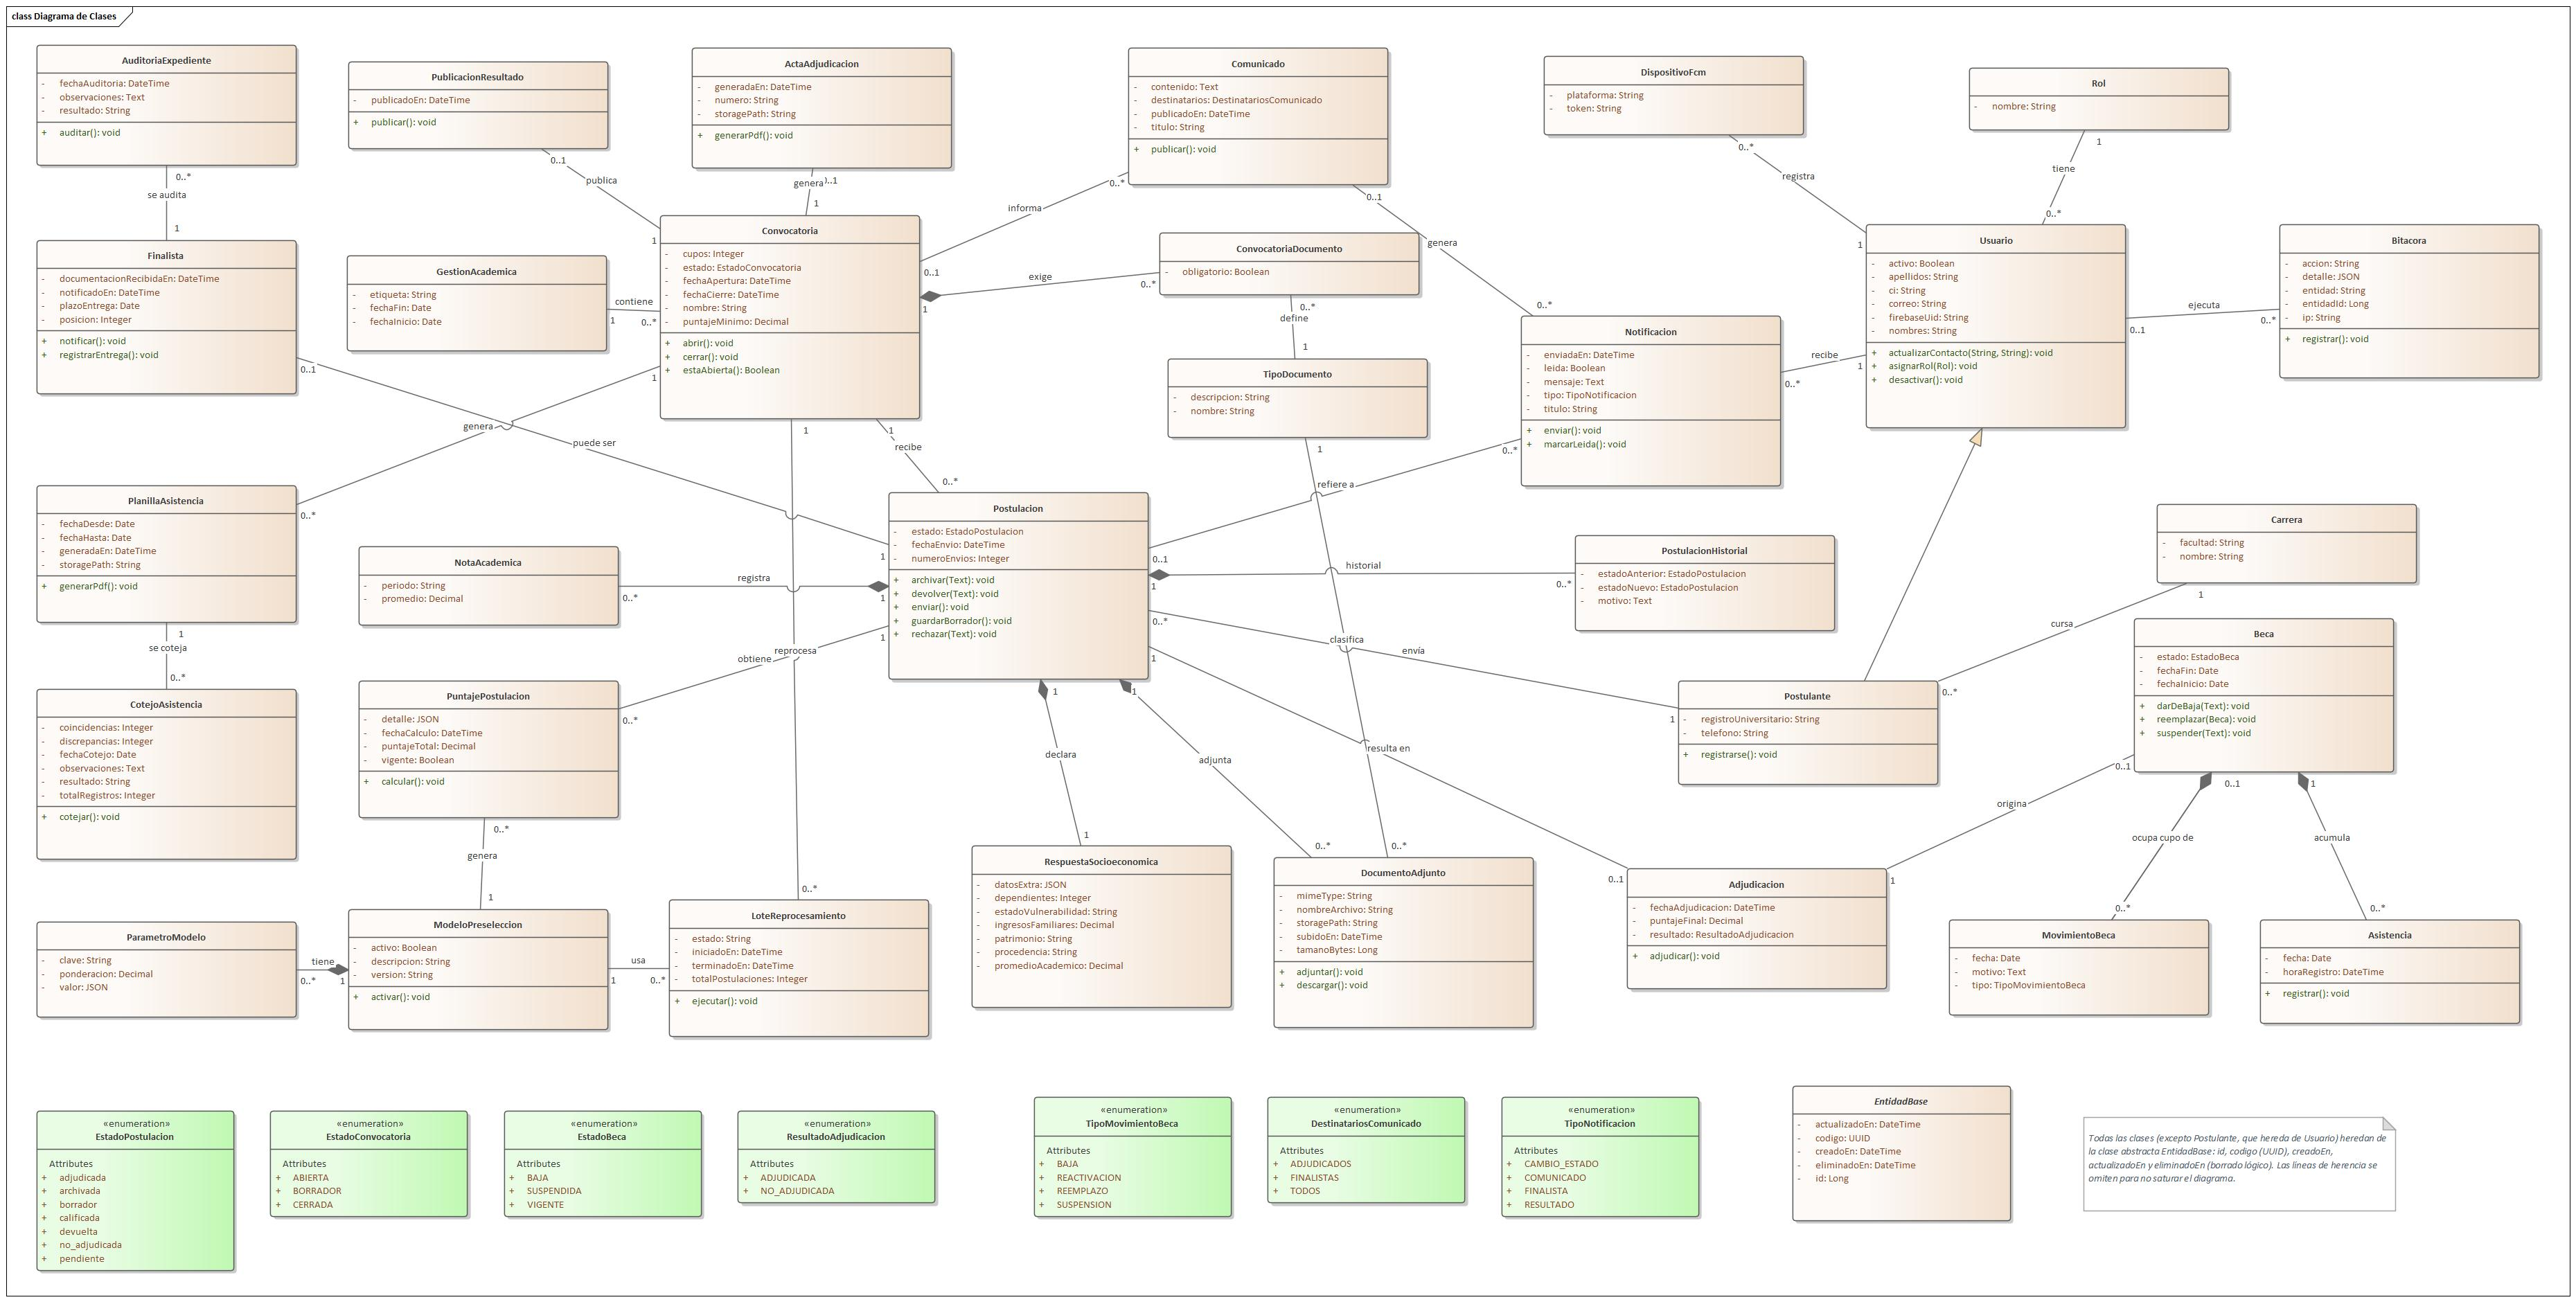
\includegraphics[width=\linewidth,height=0.8\textheight,keepaspectratio]{images/090_Diagrama_de_Clases.jpg}

\smallskip
\noindent\raggedright\textit{Nota.} Elaboración propia.
\end{figure}
\end{landscape}
